%%%%%%%%%%%%%%%%%%%%%%%%%%%%%%%%%%%%%%%%%%%%%%%%%%%%%%%%%%%%%%%%%%%%%%%%%%%
%
% Template for a LaTex article in Slovak.
%
%%%%%%%%%%%%%%%%%%%%%%%%%%%%%%%%%%%%%%%%%%%%%%%%%%%%%%%%%%%%%%%%%%%%%%%%%%%

\documentclass{article}

\usepackage[utf8]{inputenc}
\usepackage[slovak]{babel}
\usepackage[document]{ragged2e}
\usepackage{amsmath}
\usepackage{siunitx}
\usepackage{multicol}
\usepackage{textcomp}
\usepackage{amsmath, amsthm, amsfonts}
\usepackage{graphicx}
\usepackage{url}

% Theorems
%-----------------------------------------------------------------
\newtheorem{thm}{Theorem}[section]
\newtheorem{cor}[thm]{Corollary}
\newtheorem{lem}[thm]{Lemma}
\newtheorem{prop}[thm]{Proposition}
\theoremstyle{definition}
\newtheorem{defn}[thm]{Definition}
\theoremstyle{remark}
\newtheorem{rem}[thm]{Remark}

% Shortcuts.
% One can define new commands to shorten frequently used
% constructions. As an example, this defines the R and Z used
% for the real and integer numbers.
%-----------------------------------------------------------------
\def\RR{\mathbb{R}}
\def\ZZ{\mathbb{Z}}

% Similarly, one can define commands that take arguments. In this
% example we define a command for the absolute value.
% -----------------------------------------------------------------
\newcommand{\abs}[1]{\left\vert#1\right\vert}

% Operators
% New operators must defined as such to have them typeset
% correctly. As an example we define the Jacobian:
% -----------------------------------------------------------------
\DeclareMathOperator{\Jac}{Jac}

%-----------------------------------------------------------------
\title{Newtonova metóda interpolácie}
\author{Miroslav Kurka\\
  \small Dept. of Biophysics\\
  \small Pavol Jozef Šafárik University in Košice\\
  \small Slovakia 
}

\begin{document}
\maketitle


\section{Úloha}

(a) Majme tabuľku nameraných dát. Nájdite Newtonov interpolačný polynóm
s doprednými diferenciami. Upravte ho na tvar $P(x)=a_0+a_1x+a_2x^2+...+a_nx^n$ 
a porovnajte s aproximačným polynómom 6-tého stupňa zo zadania č.1. Ako sa líšia?
\begin{center}
\begin{tabular}{ |c|c|c|c|c|c|c|c|} 
 \hline
 $t_i$ & 2 & 2.5 & 3 & 3.5 & 4 & 4.5 & 5 \\
 $y_i$ & 7.14 & 6.56 & 5.98 & 5.55 & 5.71 & 6.01 & 6.53 \\
 \hline
\end{tabular}
\end{center}

(b) Generujte maticu náhodných čísiel 1000 krát 1000 $(A=rand(1000,1000))$
a vypočítajte hodnotu polynómu $P(A)$ jednak priamo a jednak pomocou Hornerovej
schémy. Porovnajte rýchlosť výpočtov s využitím príkazov tic a toc.
\subsection{Teória}\label{sec:nothing}
Majme tvar polynomu: $$N_p=C_0+C_1(x-x_0)+C_2(x-x_0)(x-x_1)+...+C_n(x-x_0)...(x-x_{n-1})$$ 
Tento polynóm definujeme ako Newtonov
polynóm. Pri riešení úlohy dosadzujeme interpolačné body do polynómu. Na získanie správneho polynómu potrebujeme zistiť koeficienty.
V jednoduchšiom prípade ak interpolačné body sú navzájom vzdialené tou istou vzdialenosťou $h$, nazyvame ich ekvidištančné a je možné využiť metódu dopredných diferencií, kde postupne výpočítavame dopredné diferencie spôsobom $\Delta y_0=y_1-y_0, \Delta^2y_0=\Delta y_1 - \Delta y_0, \Delta^2y_1=\Delta y_2 - \Delta y_1$. Následne dosádzame tieto hodnoty do $C_i=\frac{\Delta^iy_0}{i!(x_1-x_0)^i}$. Takto získame koeficienty pre náš polynóm.\cite{Bsp}
\subsubsection{Algoritmus}\label{sec:nothing2}
V prvom kroku inicializujeme maticu dopredných diferencií, kde prvý stĺpec sú hodnoty $y_i$.
Daľej napĺňame maticu do trojuholníkového tvaru, ten dosiahneme indexovanim cez druhú for slučku
od 1 po $n-j+1$, kde +1 je kvôli indexovaniu matlab polí od 1. V ďalšom kroku inicializujeme pole koeficientov a faktoríal cez vsatvanú funkciu. Následne napĺňame pole koeficientov, prvá hodnota je zo vzorca rovná $y_1$, ďalej cez for slučku výpočítavame daľšie hodnoty podľa vzorca $C_i=\frac{\Delta^iy_0}{i!(x_1-x_0)^i}$, kde -1 sú opäť kvôli indexácií. Z balíčka \emph{symbolic} využijeme funkciu \emph{syms}, ktorá slúži na definíciu funkcií. Zadefinujeme newtonov polynóm s doplnenými koeficientami a interpolačnými bodmi. Funkciou simplify zjednodušíme. Funkciou \emph{matLabFunction} "castneme" typ premennej do function handle, tento krok je potrebný na druhú časť zadania. V druhej časti
vytvoríme maticu 1000x1000 náhodných čísel. V prvom kroku prechádzame maticu a dosadzujeme cez dor slučky čísla do polynómu, kde funckiou feval výpočítavame polynóm. V druhom kroku robíme to isté len využívame funckiu horner na úpravu polynomu do hornerového tvaru. Pri obidvoch metódach meriame čas pomocou tic toc funckie 

\subsection{Výsledky}\label{sec:nothing}
Z grafu vidíme, že interpolačný polynóm prechádza presne bodmi v čom sa líší s polynómom z prvého zadania. Polynóm LSM\footnote{Polynóm v grafe nie je z dôvodu, že mi nepresne vychádza v prvej úlohe.} z prvého zadania neprechádza presne zadanými bodmi, jedná sa o aproximáciu nie o interpoláciu. Newtonov polynóm prechádza bodmi ale má napríklad nevýhodu vlnivosti. 
\begin{figure}[!htb]
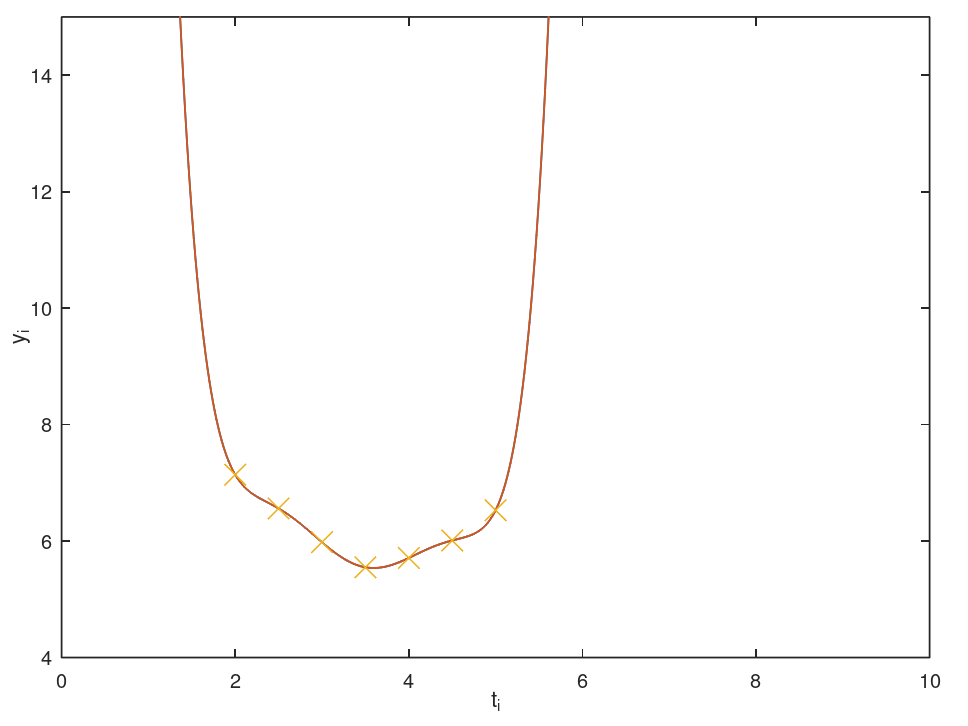
\includegraphics[scale=0.5]{graphnw.png}
\centering
\end{figure}
Pri meraní rýchlosti výpočtov ak je veľkosť matice 10x10 tak je rozdiel metód pár stotín sekúnd avšak ak je veľkosť matice 1000x1000 rozdiel časov je razantný. Pre klasický výpočet je to 17.6557 sekúnd. Pre výpočet cez hornerov tvar je tento čas zredukovaný na 0.000777006 sekúnd.

\subsection{Záver}\label{sec:nothing}
Dosiahli sme dostatočne presného Polynómu na interpoláciu našich dát. Rozdiel medzi LSM a Newtonovou metódu je v prístupe metód k bodom zadaných dát. Pri skumaní rýchlosti výpočtov bolo zistené, že za pomoci horneroveho tvaru polynómu je dosiahnúté výrazné zrýchlenie a to z dôvodu, že pri hornerovom tvare zredukujeme počet násobení z $(n^2 + n)/2$ na $n$ násobení\cite{wiki}.  
% Bibliography
%-----------------------------------------------------------------
\begin{thebibliography}{99}
\bibitem{Bsp} Buša, J., Pirč, V. and Schrötter, Š. (no date) \emph{Numerické metódy, pravdepodobnosť a matematická štatistika}, p. 263.
\bibitem{wiki} \url{https://en.wikipedia.org/wiki/Horner%27s_method#Efficiency}

\end{thebibliography}

\end{document}
